\documentclass{article}
\usepackage[utf8]{inputenc}
\usepackage{geometry}
\geometry{top=75px, bottom=75px, left=65px, right=65px}
\usepackage{amsmath}
\usepackage{amssymb}
\usepackage{algorithm}
\usepackage{algorithmic}
\usepackage{indentfirst}
\usepackage{setspace}
\onehalfspacing
\usepackage{url}
\usepackage{hyperref}
\newcommand\tab[1][1cm]{\hspace*{#1}}
\usepackage{listings}
\usepackage{xcolor}
\usepackage{changepage}
\usepackage{graphicx}
\usepackage[pages=some]{background}

\renewcommand{\baselinestretch}{1.15}

\hypersetup{
    colorlinks=true,
    linkcolor=black,
    filecolor=magenta,
    urlcolor=blue,
}

\lstset
{
    breaklines=true,
    breakatwhitespace=true,
    frame=single,
    columns=fullflexible,
    basicstyle=\ttfamily,
    showstringspaces=false,
    %numbers=left,
    %stepnumber=1,
    %numbersep=8pt,
}

\backgroundsetup{
scale=1,
color=black,
opacity=0.05,
angle=10,
position={12cm,-22cm},
contents={%
  
\includegraphics[height=20cm,width=20cm,keepaspectratio]{images/sceau.jpg}
  }%
}

%\newcommand\tab[1][1cm]{\hspace*{#1}}
\newcommand\bld[1]{\textbf{#1}}
\newcommand\ita[1]{\textit{#1}}
\newcommand\pcw[1]{\texttt{#1}}

\begin{document}
\begin{titlepage}
    \begin{center}
        \BgThispage
        \vspace*{1cm}
        
        
        \huge
        \textbf{Data Warehouses}
        \vspace{0.25cm}
        
        \LARGE
        \textbf{INFO-H419}
        
        \vspace{0.5cm}
        \LARGE
        {Part 2 : TPC-DI benchmark on Impala}
        
        
        \vspace{3.5cm}
        
        \textbf{BAKKALI Yahya (000445166) \\}
        \textbf{FALLAHI Amirmohammad (000460073) \\}
        \textbf{HAUWAERT Maxime (000461714) \\}
        \textbf{LIBERT Alexandre (000435755) \\}
    
        \vspace{2.5cm}
        \textit{December 2021 \\}
        \vspace{0.5cm}
        \textsc{Université Libre de Bruxelles (ULB)}
        
        
    \end{center}
\end{titlepage}

\tableofcontents
%\thispagestyle{empty}
\newpage
%\setcounter{page}{1}
\setlength{\parskip}{1em}

\section{Introduction}

The ongoing demand for modernisation in nowadays societies, have been obliged the data warehouse tools to supply high efficiency. In order to provide high efficiency, the \bld{data integration} process of these tools can play an effective role.

Following the first part of the project, in this part also \bld{TPC} tools have been used to verify efficiency of \bld{Impala}. For this part of project, \bld{TPC-DI} benchmark have been exploited; TPC-DI is a benchmark for data integration. In this paper the details of the TPC-DI experiment, performed on Impala, will be explained.

\section {Data Integration \& ELT}
\bld{Data integration} is set of processes in which data from several sources will be combined in order to create a connected, single view of data. \bld{ETL} is a 3-step operation in order to Extract, Transform and Load data into the data warehouse. In fact ETL process can be used in order to integrate data. During ETL process the is collected from an initial system, then it will be converted into analyzable format, and placed into a data warehouse. 

\vspace{0.5cm}
\begin{figure}[H] 
\begin{center}
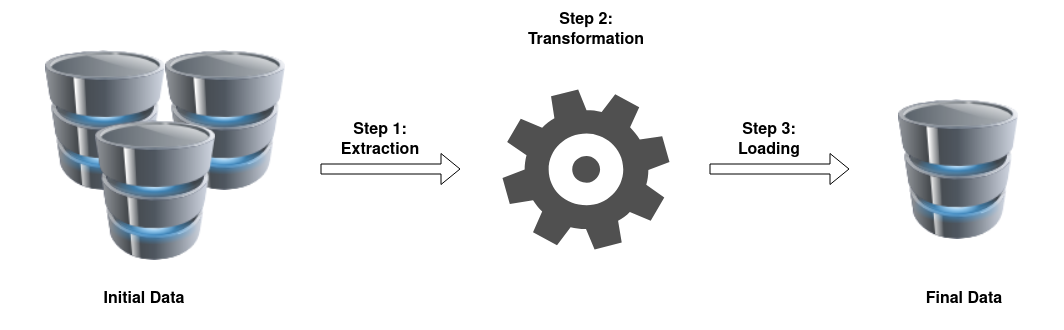
\includegraphics[width=15cm, height=5cm]{images2/etl.png}
\end{center}
\caption{ETL process}
\label{etl}
\end{figure}


The ETL steps can be defined as follow:
\begin{enumerate}
    \item \bld{Extraction: } In this step data will be extracted from different sources and will be stored in a "staging area" in order to avoid disorder in initial sources. This step validate the data and ensure that the data is accurate. At this stage, unnecessary data is removed, duplicates are identified and deleted. The data type is also examined and modified.
    \item \bld{Transformation: } Data extracted from data sources are raw and usually not ready for use and analysis. Raw data at this stage must be cleared and converted to the required format. This step is key step of ETL as it transform raw data to valuable and usable data. Second phase of data validation is also checked at this stage. If it is necessary to merge columns or separate columns and convert them into several columns, this will be done in this step.
    \item \bld{Loading: } Loading data to the data warehouse is the last step in the ETL process. Usually a large amount of data must be loaded in a short time (overnight) in the data warehouse, so it is very important to pay attention to performance optimisation. The data loading process may also fail and stop during execution. The recovery operation must be performed exactly from the stop point and the necessary actions must be taken to prevent non-integration and duplication or loss of data. At this stage, the necessary strategies to deal with such events must be planned. 
\end{enumerate}


\section{Hardware specification}
In fact, the same computer (\ita{Dell xps-15-9560}) as the first part has been used in order to perform the TPC-DI benchmark experimentation. The following table shows the hardware specification of this computer. 
\newline
\begin{table}[h]
\centering
\begin{tabular}{|l|c|}
\hline
Operating system & Ubuntu 20.04.3 LTS \\ \hline
System type & 64 bits \\ \hline
CPU & Intel®Core™i7-7700HQ \\ \hline
CPU frequency & 2.8 GHz up to 3.8 GHz \\ \hline
RAM capacity & 16 GB \\ \hline
RAM type & DDR4 \\ \hline
RAM speed & 2,400 MT/s \\ \hline
Hard disk & PM981 NVMe Samsung \\ \hline
Hard disk capacity & 256 GB \\ \hline
\end{tabular}
\caption{Device information}
\label{table:Table 1}
\end{table}


\section{Software Specification}

As in the first part of the project, Impala structure and functionality have been described in details, in this paper these kinds of description have been ignored. So in this section, the TPC-DI tool will be verified.

\subsection{TPC-DI}
In this first part of the project, TPC-DS experiment has been performed on Impala; In this part, the TPC-DI experiment will be verified. 

\bld{TPC-DI} is a benchmarking test for technologies that transform and integrate data between systems. The benchmark procedure prepares data for utilization in a Data Warehouse by arranging a specified size of data. Data from an On-Line Transaction Processing (OTLP) system is transformed, together with data from other sources, and fed into a Data Warehouse in the benchmark model. The benchmark tests a wide range of system components related with data integration contexts, which would include:
\begin{itemize}
    \item The loading and processing of enormous amounts of data
    \item A combination of transformation types like error checking, data type conversion, etc.
    \item Historical loading and cumulative updates of a target Data Warehouse using the transformed data
    \item Several data sources in various forms 
    \item Other useful tests
\end{itemize}
The operations of the TPC-DI are represented as follows:
\begin{itemize}
    \item TPC supplied code is used to produce source data. The data is transferred as flat files, similar to what many extraction programs provide.
    \item The data transformation process starts with the reading of the Source Data by the System Under Test (SUT).
    \item The transformations ensure that the Source Data is accurate and that the data is appropriately structured before being loaded into a Data Warehouse.
    \item When all Source Data has been transformed and is available in the Data Warehouse, the process is complete.
\end{itemize}

\subsubsection{TPC-DI experimentation method}
In order to illustrate better the experimentation method, the photo of official documentation of TPC-DI has been used. In fact the figure \ref{tpcdi} illustrates the TPC-DI benchmark modelisation. Let's verify this model:
\begin{figure}[H] 
\begin{center}
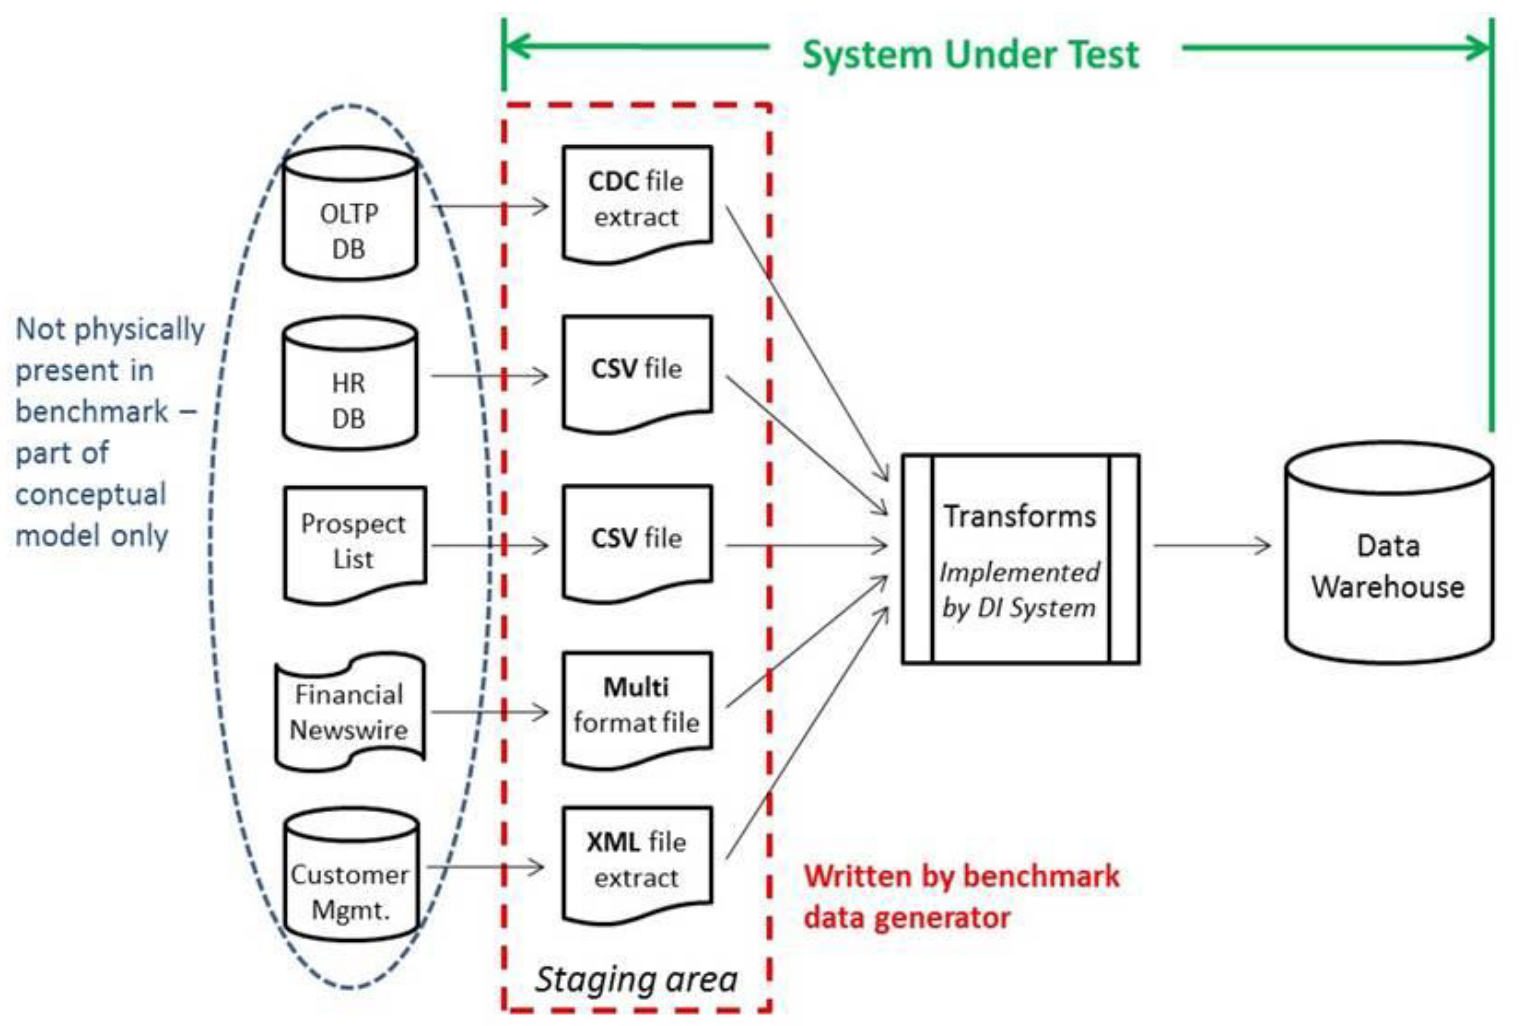
\includegraphics[width=15cm, height = 8cm]{images2/tpcdi2.png}
\end{center}
\caption{TPC-DI benchmark model}
\label{tpcdi}
\end{figure} 

As the figure shows, first the data is extracted from source databases and added to staging area, then the transformation begins on extracted data and finally the transformed data will be loaded on data warehouse. The procedure of extracting files from data sources to the staging area is not tested by the TPC-DI because it uses its generative scripts to produce these files automatically. 

As it has been explained in the previous sections, the key phase of ETL process is transformation. In this phase, unnecessary columns will be removed, different kinds of definition for same data will be homogenised, the units will be unified and in general converting data from character representations to data types that comply with the Data Warehouse standard.

Developing a data warehouse for commercial or scientific exploitation, consists of two main phases:
\begin{itemize}
    \item \bld{Historical load:} Which is simply  the record of already existed data, for instance the transactions of previous years.
    
    \item \bld{Incremental update:} Which is the technique of loading data progressively. The destination database only receives new and modified data. Non-changing data will be left alone. 
\end{itemize}

In this project, only \ita{historical load} phase has been verified.

Now let's take a look at the figure which has been provided by TPC-DI official documentation for the destination data model.

\begin{figure}[H] 
\begin{center}
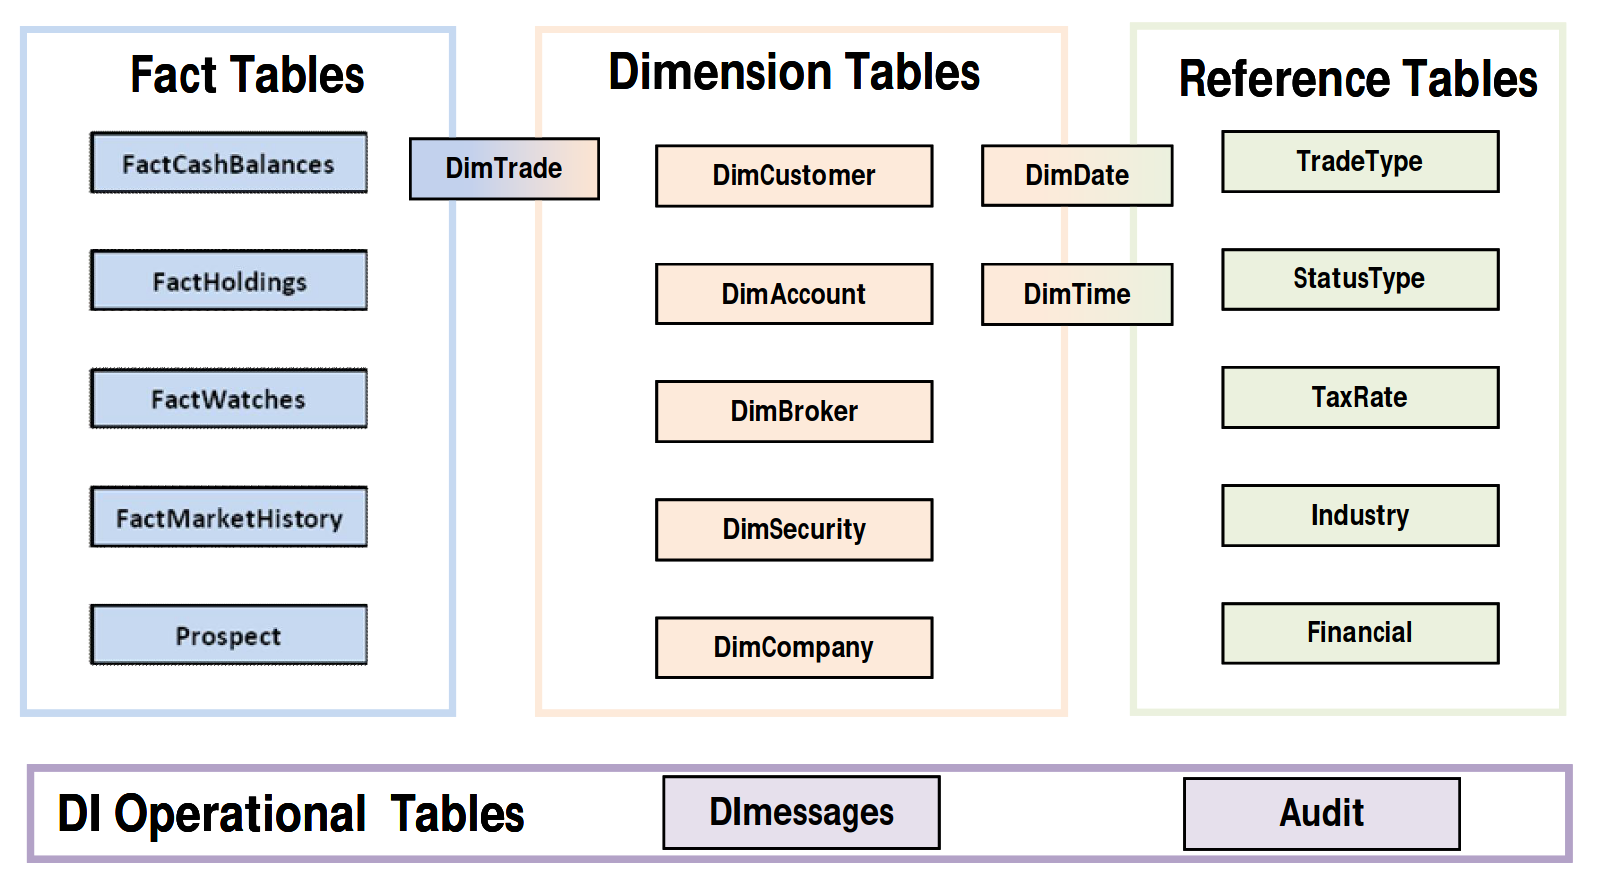
\includegraphics[width=15cm, height=8cm]{images2/destmodel.png}
\end{center}
\caption{Destination Data Model}
\label{dstmdl}
\end{figure} 

A dimensional data warehouse is where the TPC-DI workload ends up. Dimensional models are widely used in the industry and are meant to provide quick answers to a number of business concerns. There are numerous methods to create a data warehouse, however this format gives a well-understood structure in the benchmark Data Warehouse while also allowing the TPC-DI workload to apply a diverse set of data transformations. 

According to TPC-DI official documentation, in a dimensional model, dimension tables defines the business entities of interest and fact tables provide measurement data about what happened, such as the price and volume of a transaction. 

\subsection{Apache Impala vs Apache Hive}
Hadoop, main component, is HDFS (Hadoop Distributed File System) and MapReduce. MapReduce involves breaking into small batches a large volumes of data, and then process them separately
In the TPC\_DS project we saw how to install and run Impala.

\subsubsection{MPP vs MapReduce}
\textit{
MPP and MapReduce are used in different scenarios.
MPP is used on expensive, specialized hardware tuned for CPU, storage and network performance. MapReduce and Hadoop find themselves deployed to clusters of commodity servers that in turn use commodity disks. The commodity nature of typical Hadoop hardware (and the free nature of Hadoop software) means that clusters can grow as data volumes do, whereas MPP products are bound by the cost of, and finite hardware in, the appliance and the relative high cost of the software.}
\footnote{\url{https://www.zdnet.com/article/mapreduce-and-mpp-two-sides-of-the-big-data-coin/}}


\subsubsection{Impala vs Hive Queries}
\textit{Hive queries translate to MapReduce jobs. Impala queries implement memory bound MPP jobs that are much faster than disk based MapReduce. Unlike Hive, Impala doesn't rely on data transformations or moving data to process queries. Impala also avoids startup overhead by starting daemon processes at boot time. This makes Impala more readily available to process queries than Hive since Hive has to start new processes for every query you run.
Since Hive is MapReduce based, it adds a level of fault-tolerance that Impala can't match. While Impala makes querying a lot faster, it loses the added advantage of fault-tolerance provided by Hadoop MapReduce jobs.}
\footnote{\url{https://www.stackchief.com/blog/Hive\%20vs\%20Impalal}}


\subsubsection{Read Only Schema}
\textit{Hive is “Schema on READ only“. So, functions like the update, modifications, etc. don’t work with this. Because the Hive query in a typical cluster runs on multiple Data Nodes. So it is not possible to update and modify data across multiple nodes.(Hive versions below 0.13)}\footnote{\url{https://www.guru99.com/introduction-hive.html}}

\subsubsection{Impala no Update}
As explained, the idea of read-only in Hive also applies to Impala. That' s why, in this project, we could not perform any data update in the tables.

\subsection{Pentaho Data Integration}

Pentaho is a piece of software which allows everyone to perform business intelligence tasks on large quantities of data. It covers the common areas of ETL, reporting, OLAP/analysis and data mining. The software is developed since 2004 entirely in Java which allows cross-platform support for the popular operating systems, at the beginning by Pentaho Corporation, then Pentaho was acquired by Hitachi Data Systems in 2015. \footnote{\url{https://www.hitachivantara.com/en-us/company.html}}

\subsubsection{Introduction to Pentaho}

Pentaho Data Integration\footnote{\url{https://help.hitachivantara.com/Documentation/Pentaho/5.2/0J0/0C0/000}}(PDI) is a software of Pentaho which performs data integration. It is an ETL solution which means that it can extract, transform and load data from various sources. Pentaho also provides a desktop application called Spoon, which allows anyone to perform these tasks with an intuitive graphical interface(the PDI desktop is called Spoon).

%PDI includes the DI Server, a design tool, three utilities, and several plugins.


\subsubsection{Use cases}
Pentaho Data Integration(PDI) is suitable for several use cases\footnote{\url{https://help.hitachivantara.com/Documentation/Pentaho/5.2/0J0/0C0/000}}:

\begin{itemize}
\item Having to insert large quantities of data into databases while using the full power of computation of the available pieces of hardware.
\item Having to populate a data warehouse without having problems with creating surrogate keys as well as slowly changing dimensions.
\item Having to clean or correct data with simple or complex computations.
\item Having to migrate data from one database to another.
\item Having to deal with data arriving in real-time.
\item Having to perform several Hadoop functions such scheduling and executing jobs, designing Hadoop MapReduce.
\item Having to prototype Relational OLAP schemas.
\end{itemize}

\subsubsection{PDI structure}
The Data Integration allows the use of two basic document types: 
\begin{itemize}
\item Transformations : used to describe the ETL data flows, e.g. reading input from a source file, then transforming these data and loading them into a target location(database, file, ...).
\item Jobs : used to coordinate ETL activities such as defining the order of execution of the transformations flow and dependencies, or checking for execution conditions, before execution e.g. I/O availability...
\end{itemize}

PDI transformation use two main components: 
\begin{itemize}
\item Steps : They are the building blocks, each step is designed to perfom a specific task, e.g. input/output file or database, filter rows... and more than 140 others
\item Hops : they are the data pathways between steps 
\end{itemize}

\subsubsection{Connect Cloudera Impala to Pentaho}
Impala offers connectors ``Impala JDBC Connector 2.6.X for Cloudera Enterprise" to allow connection between the database and Pentaho DI, it can be found in their official site~\footnote{\url{https://www.cloudera.com/downloads/connectors/impala/jdbc/2-6-15.html}}.
Pentaho can not insert efficiently on Impala database, it suggests to use Hadoop cluster instead.

\section{Implementation}
In this section, details of implementation and experimentation will be seen. This section shows how the input of the experimentation has been provided and also explains how the situation of the experimentation has been facilitated for users. It will also verify different level of experimentation. 

As in the first part of the project, the handling of Impala was explained in depth, we will ignore it here.

\subsection{Preparing TPC-DI environment}
Once the TCP-DI tool was downloaded from TPC official website\footnote{\url{http://tpc.org/tpc_documents_current_versions/current_specifications5.asp}}, the experimentation environment can be prepared. In this subsection, the preparation for experiment environment will be verified.

\subsubsection {Source data preparation}

The TPC-DI tool gives the possibility to create the source data; The source data will be generated by launching the following commands after extracting the file \pcw{tpc-di-tool.zip} and going to Tools directory. 
\begin{lstlisting}[language=bash]
$ mv  PDGF pdgf
$ java -jar DIGen.jar
\end{lstlisting}

\subsubsection{Data warehouse preparation}

In order to provide the data warehouse, just the file \pcw{create\_table\_fk.sql} has been launched by following command:
\begin{lstlisting}[language=bash]
$ bin/impala-shell.sh -f <path_to_the_create_tables_fk.sql>/create_tables_fk.sql
\end{lstlisting}
The result is as follows:
\begin{figure}[H] 
\begin{center}
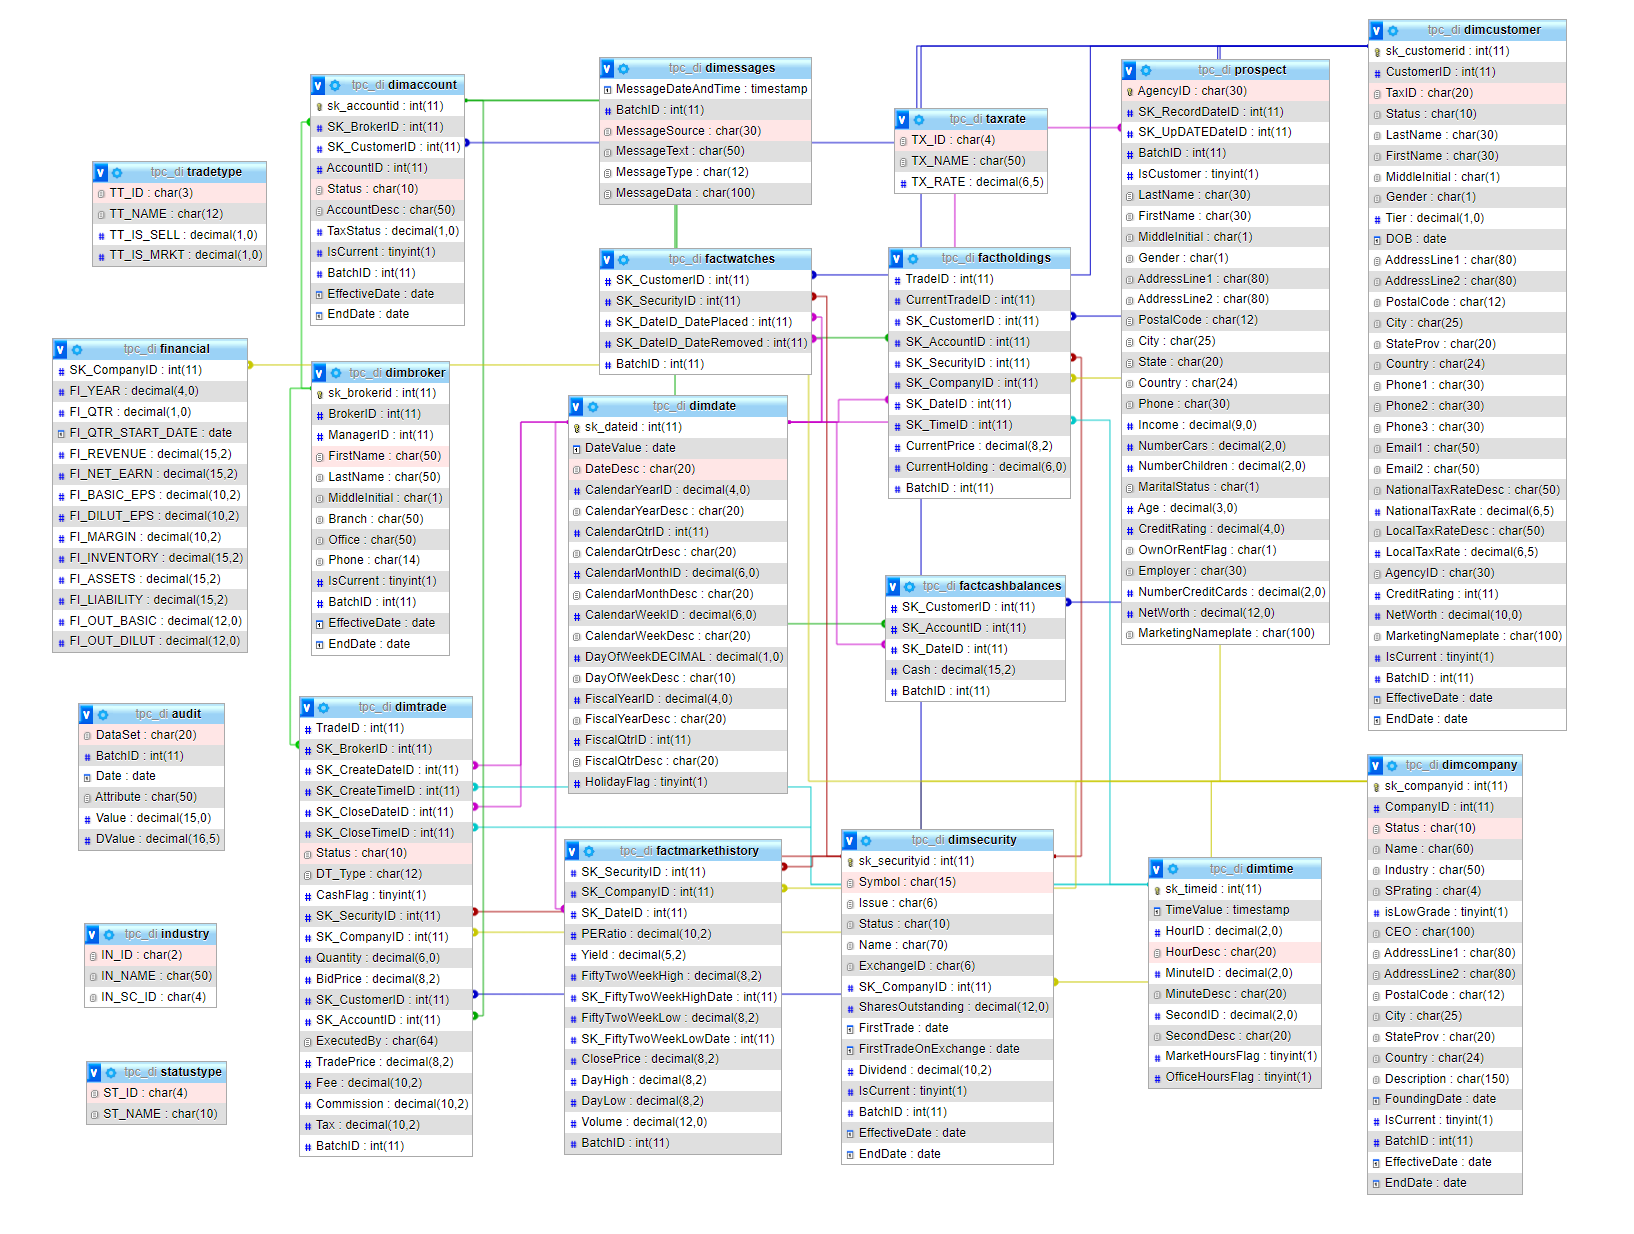
\includegraphics[width=\textwidth, height=20cm]{images2/tables.png}
\end{center}
\caption{Data warehouse}
\label{Tables}
\end{figure} 

\subsubsection{Preparing Pentaho Data Integrator}

After downloading Pentaho from the official website \footnote{https://sourceforge.net/projects/pentaho/files/latest/download}, by launching the file \pcw{spoon.sh} the Pentaho graphical user interface will be opened and will be ready to begin the experiment.




\subsection{Historical Load}

In this section, the ETL process of each table will be shown in details. There are tables which have been loaded easily, but there are also tables that their historical load depends on other tables. The complete process for historical load and the result of this process can be seen below:
\begin{figure}[H] 
\begin{center}
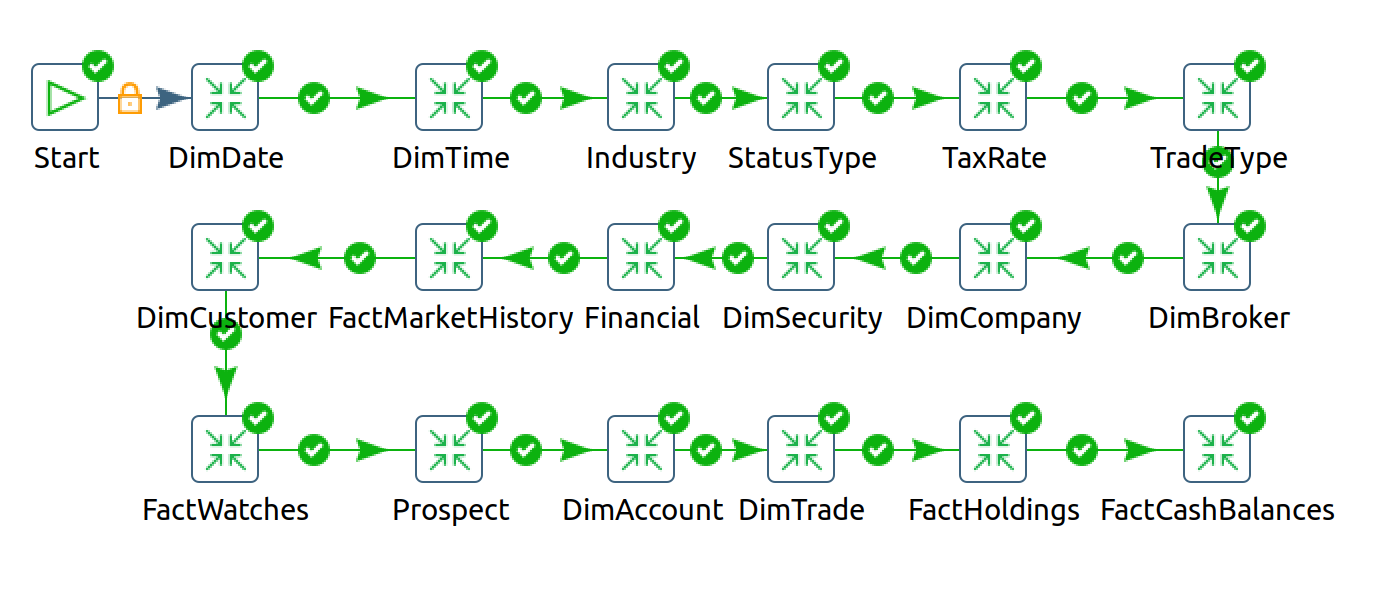
\includegraphics[width=15cm, height=5cm]{images2/ALLL.png}
\end{center}
\caption{Historical load process}
\label{DimBroker}
\end{figure} 

\begin{figure}[H] 
\begin{center}
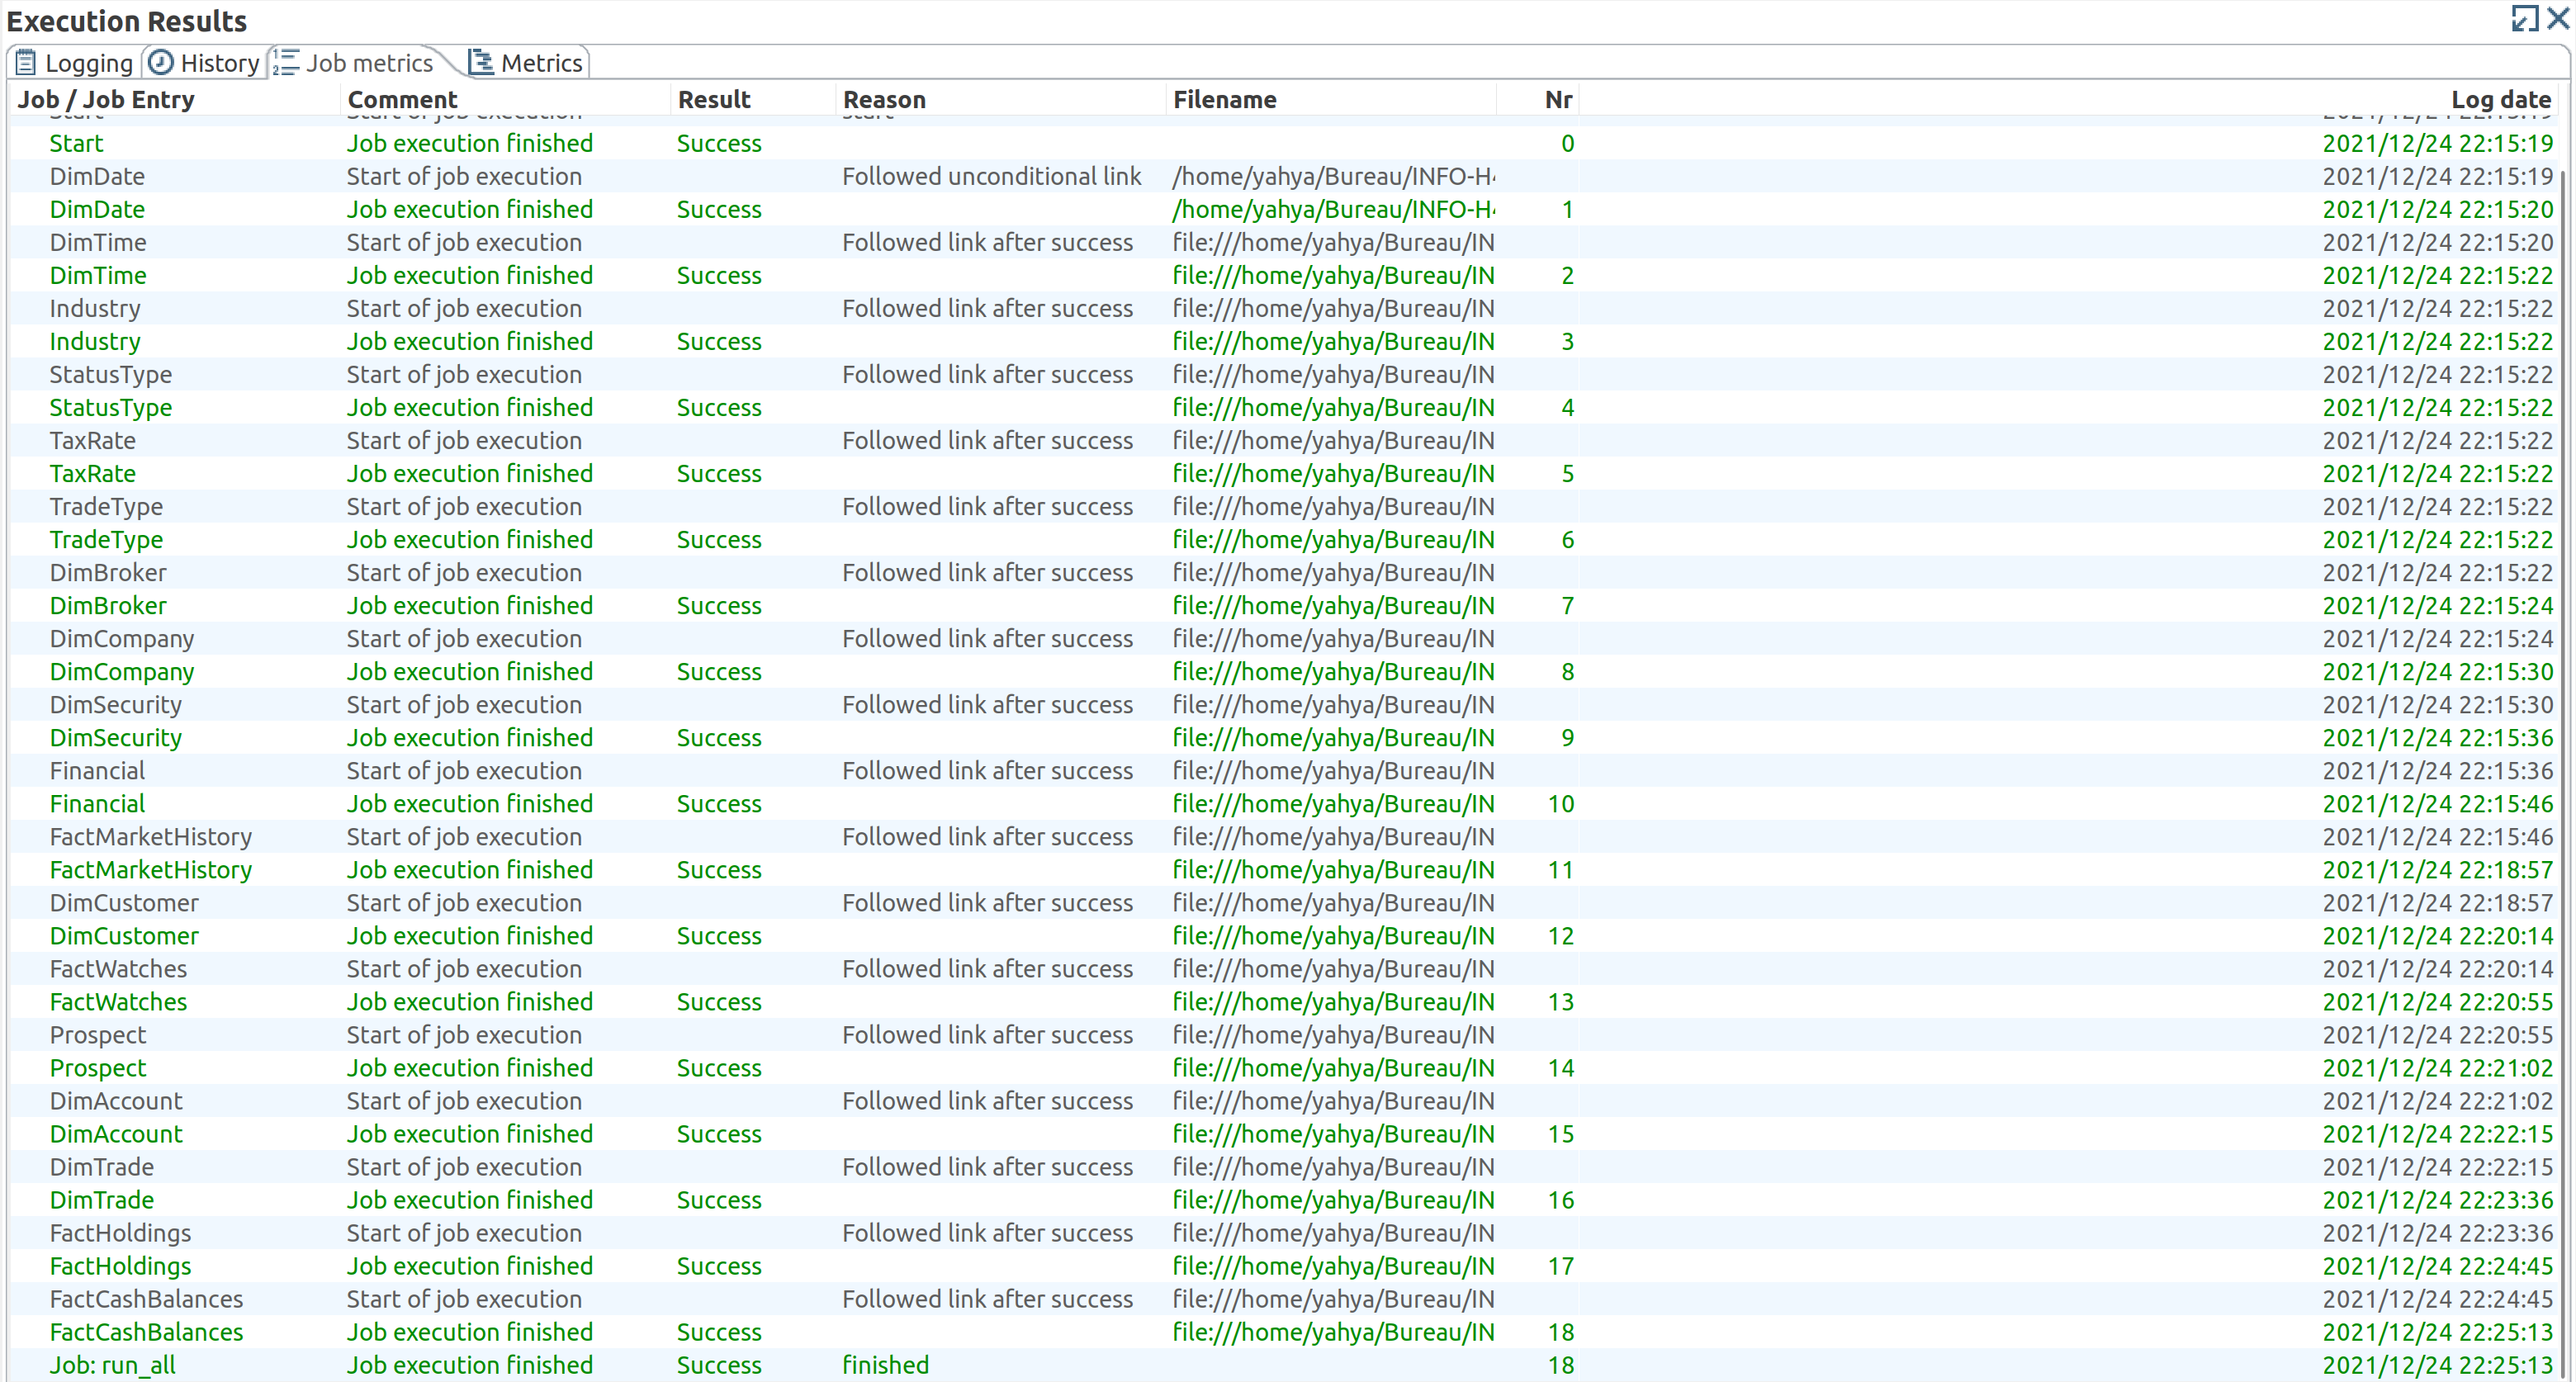
\includegraphics[width=15cm]{images2/ALLRES.png}
\end{center}
\caption{Historical load process result}
\label{DimBroker}
\end{figure} 


\subsubsection{Type read \& load}
These tables are static; The data will be read from the file and will be loaded in the destination without any modifications. Below is an example for implementation of these kinds of table:
\begin{figure}[H] 
\begin{center}
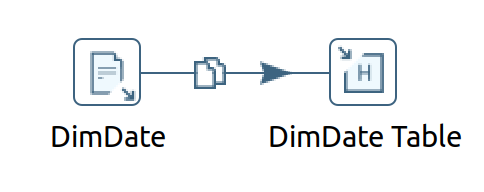
\includegraphics[width=7cm, height=2.5cm]{images2/TypeA2.png}
\end{center}
\caption{Implementation of tables type read \& load}
\label{readload}
\end{figure} 
The following tables are the tables of type read \& load:
\begin{table}[H]
\begin{center}
\begin{tabular}{|c|c|c|}
\hline
DimTime & DimDate  & StatusType \\ \hline
TaxRate & Industry & TradeType  \\ \hline
\end{tabular}
\end{center}
\end{table}

\subsubsection{DimBroker}
Data of this table have been extracted from \pcw{HR.csv} file; From this file, those employees who are brokers (EmployeeJobCode = 314) will have data copied to the Broker table.
\begin{figure}[H] 
\begin{center}
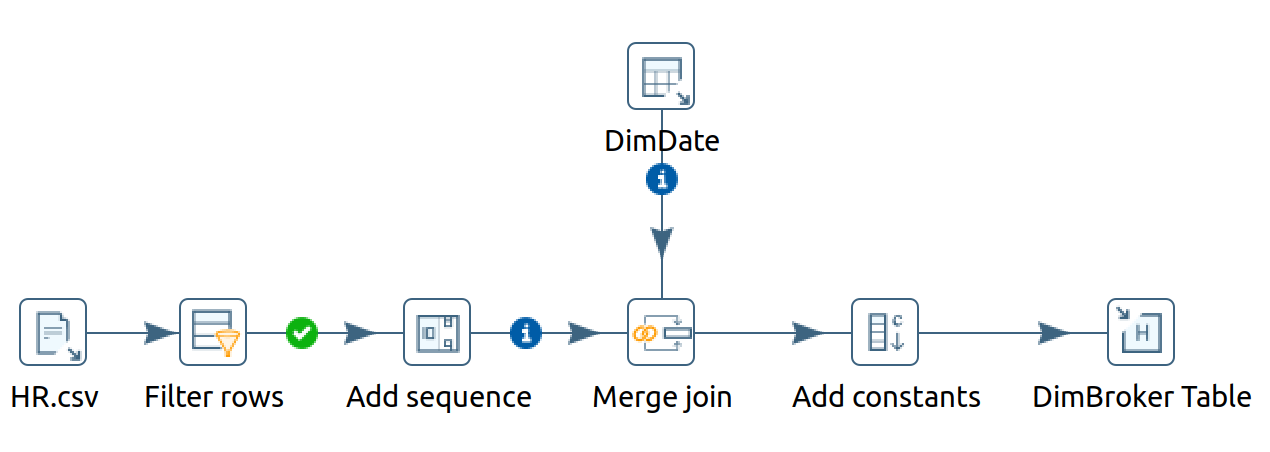
\includegraphics[width=15cm, height=2.5cm]{images2/DimBroker.png}
\end{center}
\caption{Implementation of DimBroker table}
\label{DimBroker}
\end{figure} 


\subsubsection{DimCompany}
The \pcw{FINWIRE} files are used to extract DimCompany data. The records of type CMP are used to process all \pcw{FINWIREyyyyQq} files in ascending year and quarter sequence. Notice that in its implementation also some connection with StatusType and Industry tables have been done.
\begin{figure}[H] 
\begin{center}
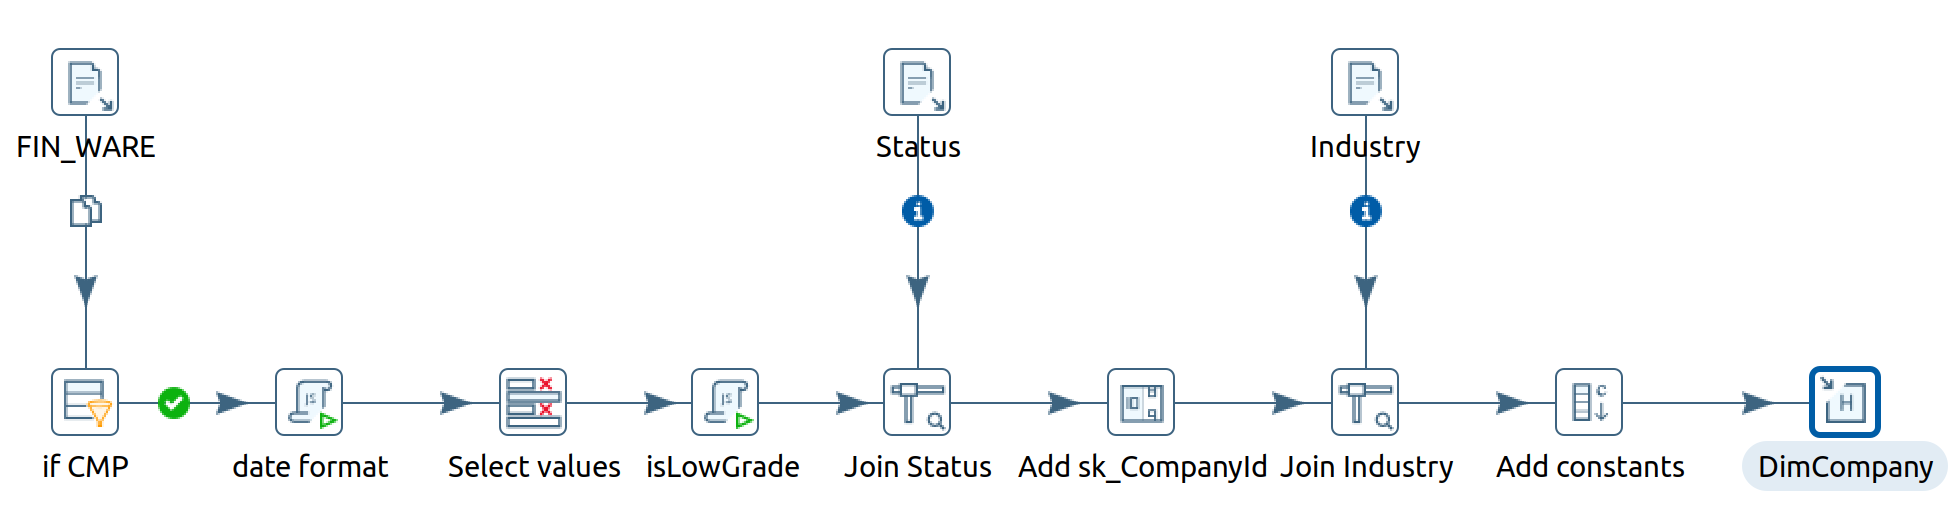
\includegraphics[width=15cm]{images2/dimcompany.png}
\end{center}
\caption{Implementation of DimCompany table}
\label{DimBroker}
\end{figure} 

\subsubsection{DimSecurity}
The \pcw{FINWIRE} files are used to extract DimCompany data. The records of type CMP are used to process all \pcw{FINWIREyyyyQq} files in ascending year and quarter sequence, and records of type SEC are used. It is linked with DimCompany and StatusType.
\begin{figure}[H] 
\begin{center}
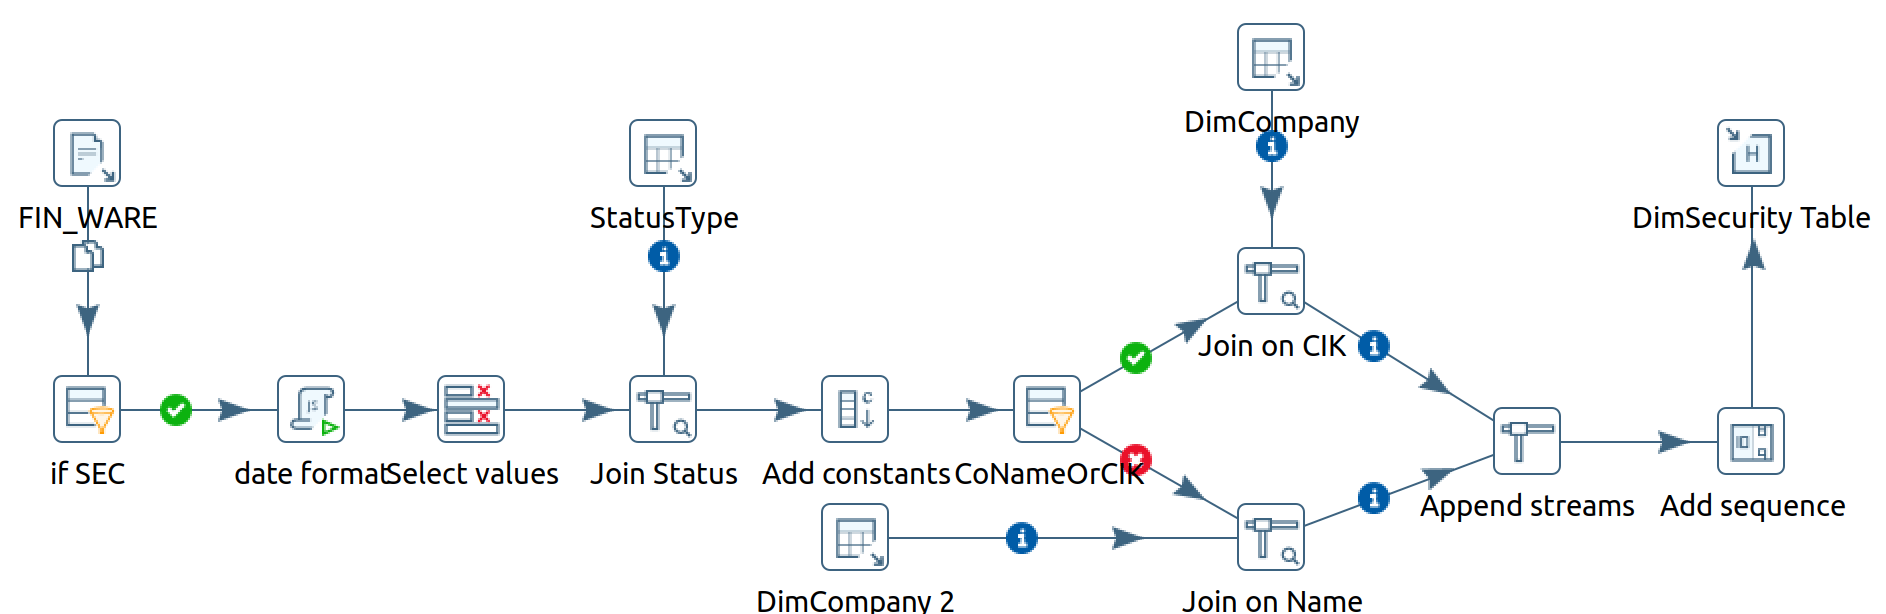
\includegraphics[width=15cm]{images2/DimSecIMP.png}
\end{center}
\caption{Implementation of DimSecurity table}
\label{DimBroker}
\end{figure} 


\subsubsection{Financial}
The \pcw{FINWIRE} files are used to extract DimCompany data. The records of type CMP are used to process all \pcw{FINWIREyyyyQq} files in ascending year and quarter sequence, and records of type FIN are used. There is a connection with DimCompany in its implementation.
\begin{figure}[H] 
\begin{center}
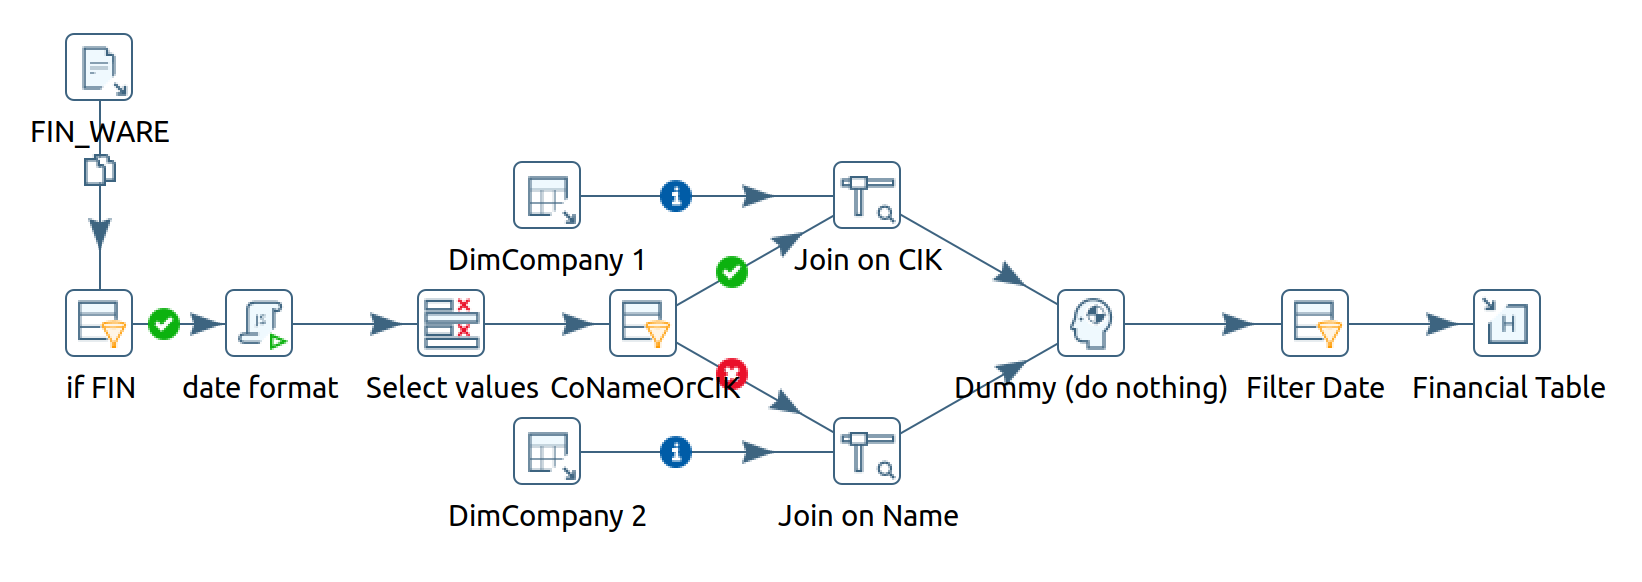
\includegraphics[width=15cm, height=4cm]{images2/FinancIMP.png}
\end{center}
\caption{Implementation of Financial table}
\label{Financ}
\end{figure} 

\subsubsection{FactMarketHistory}
The data for this table is extracted from thr file \pcw{DailyMarket.txt}. The challenging aspect for this table was grouping the entries by date and security ID while keeping the date of highest value and lowest value for both of them. As following figure shows, this problem has been handled.
\begin{figure}[H] 
\begin{center}
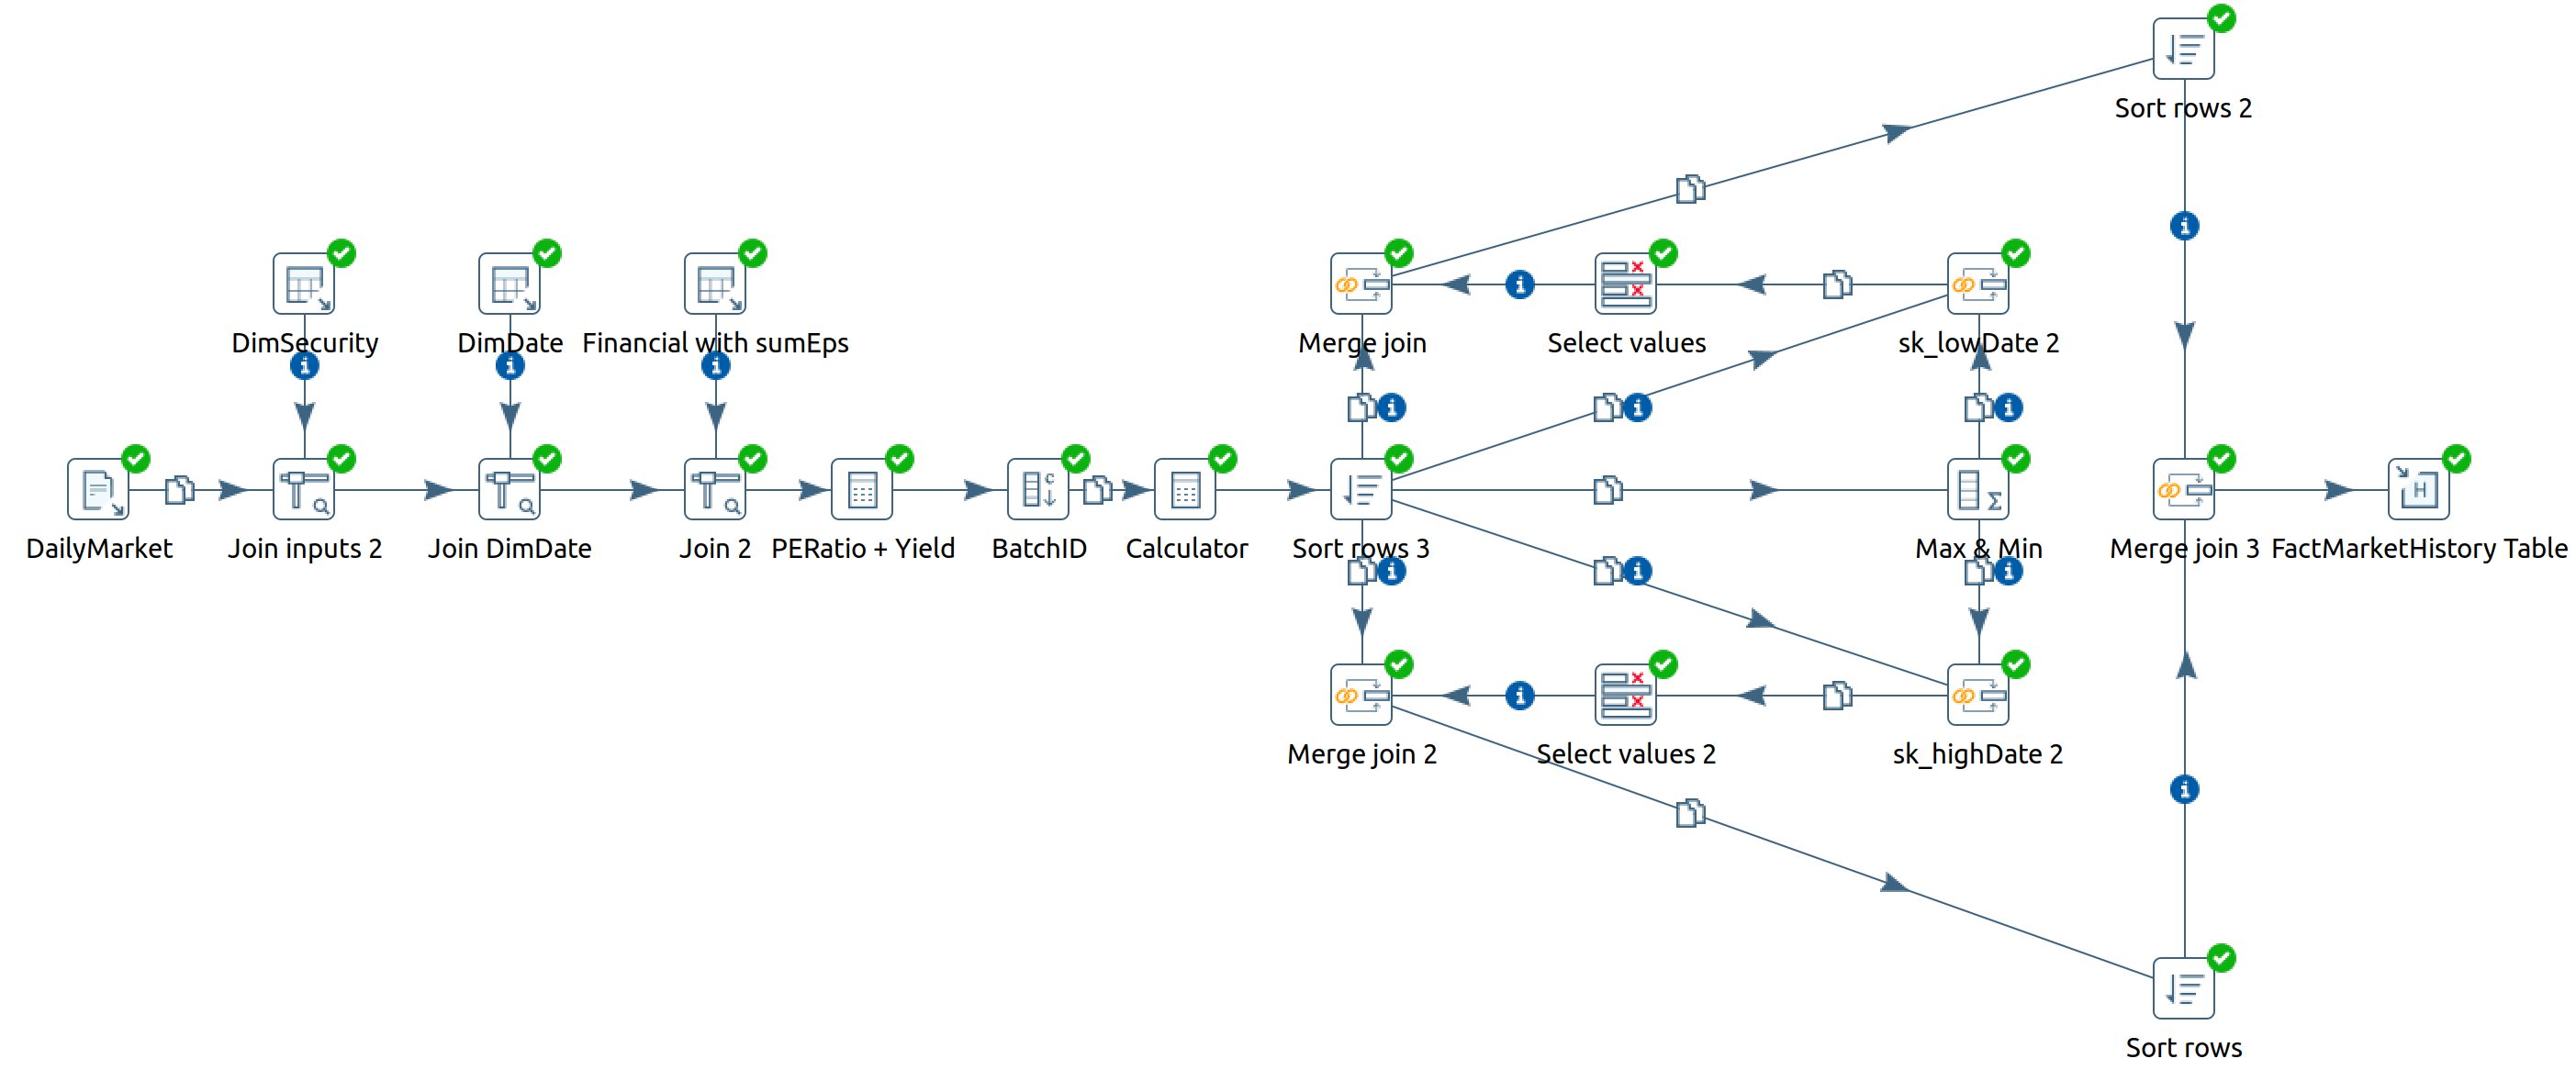
\includegraphics[width=15cm, height=12cm]{images2/FMHIMP.png}
\end{center}
\caption{Implementation of Financial table}
\label{FMHimp}
\end{figure} 


\subsubsection{DimCustomer}
The data of this table is extracted by using the file \pcw{CustomerMgmt.xml}. Customer data is kept as a sub-part of the Action element. Every action will have a Customer associated with it, but not all actions will necessitate changing the DimCustomer table.
\begin{figure}[H] 
\begin{center}
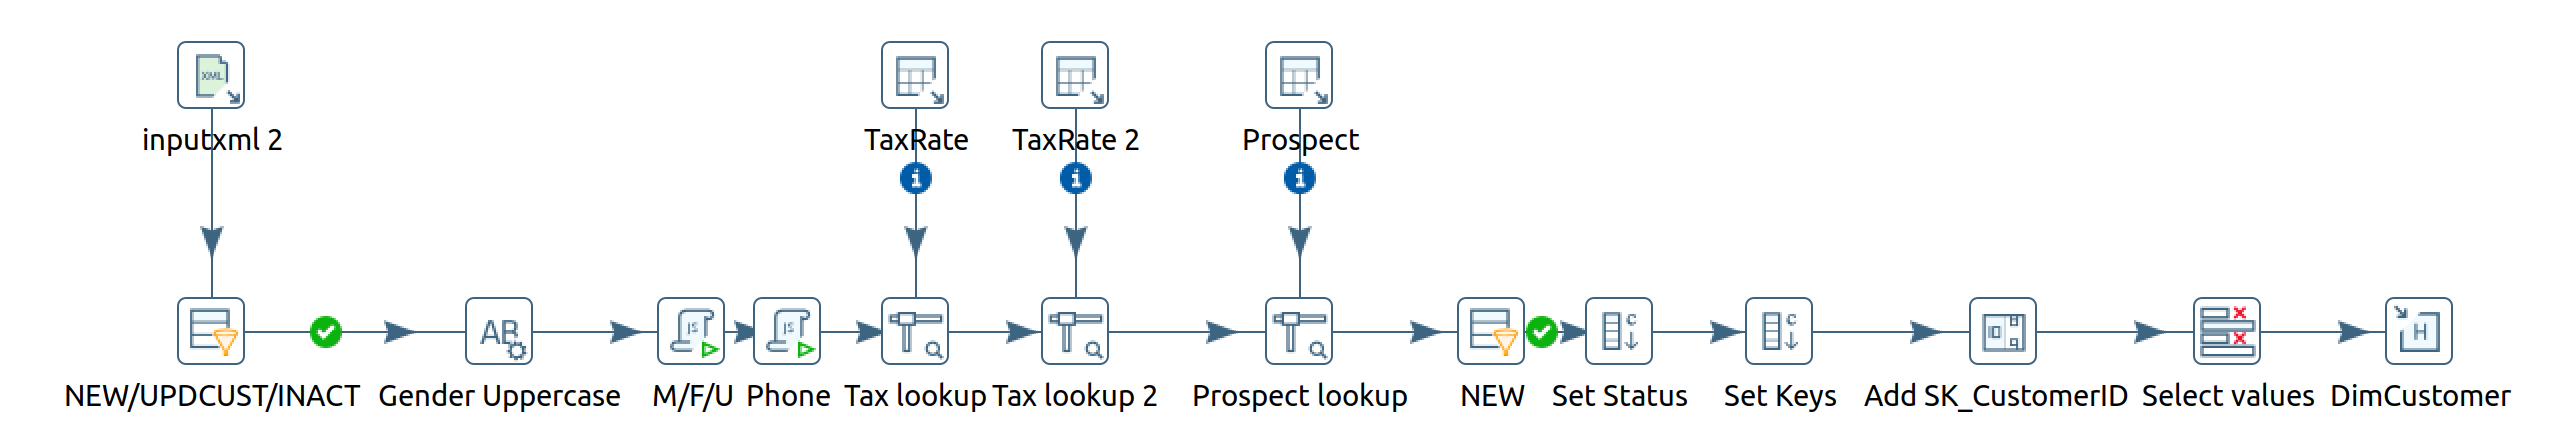
\includegraphics[width=15cm]{images2/DimCus.png}
\end{center}
\caption{Implementation of DimCustomer table}
\label{DimCus}
\end{figure} 

\subsubsection{FactWatches}
Data for FactWatches extracted from the \pcw{WatchHistory.txt} file. For the Customer, Security, and Date dimension references, surrogate keys must be acquired. The date keys show when the watch was put on and taken off. 
\begin{figure}[H] 
\begin{center}
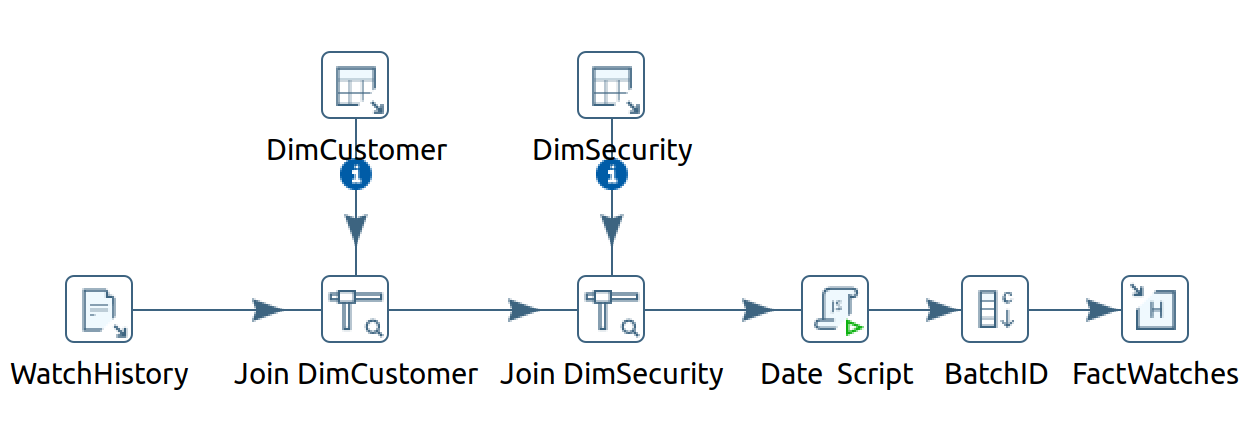
\includegraphics[width=15cm]{images2/fctWat.png}
\end{center}
\caption{Implementation of FactWatches table}
\label{fctWat}
\end{figure} 


\subsubsection{Prospect}
Prospect data have been extracted from \pcw{Prospect.csv}. The only matter to handle for this table was to verify if a customer exists (or does not). 
\begin{figure}[H] 
\begin{center}
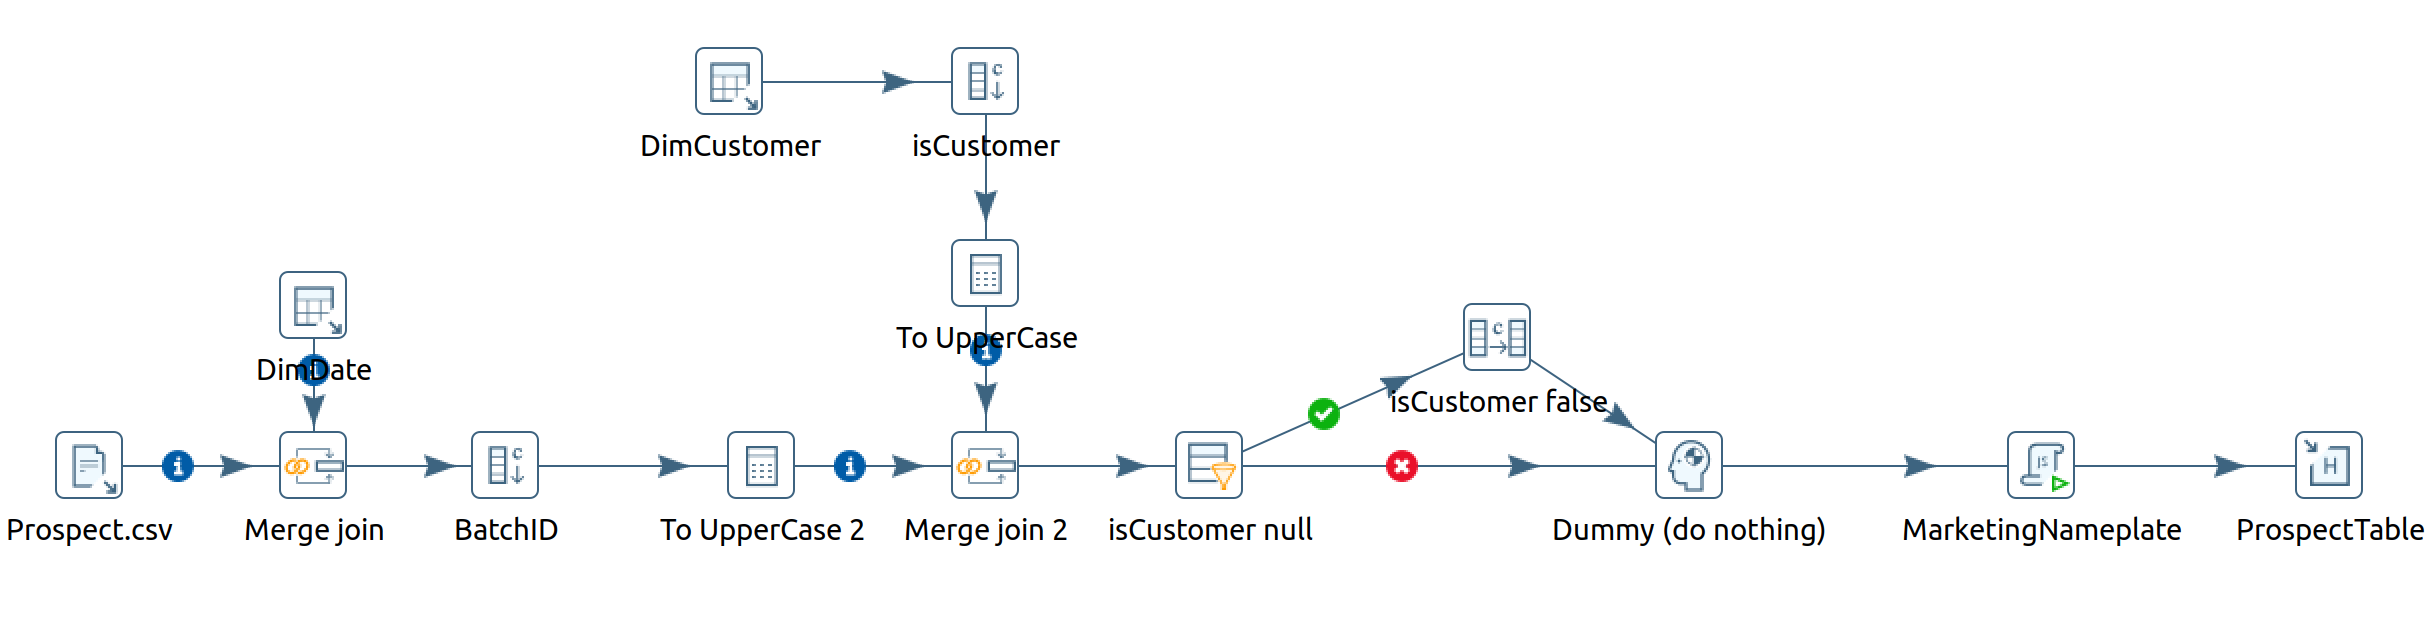
\includegraphics[width=15cm, height=6cm]{images2/Prospect.png}
\end{center}
\caption{Implementation of Prospect table}
\label{DimCus}
\end{figure} 

\subsubsection{DimAccount}
DimAccount data is also based on \pcw{CustomerMgmt.xml} like DimCustomer data; The major difference with DimCustomer is that DimAccount must be linked to the relevant broker.
\begin{figure}[H] 
\begin{center}
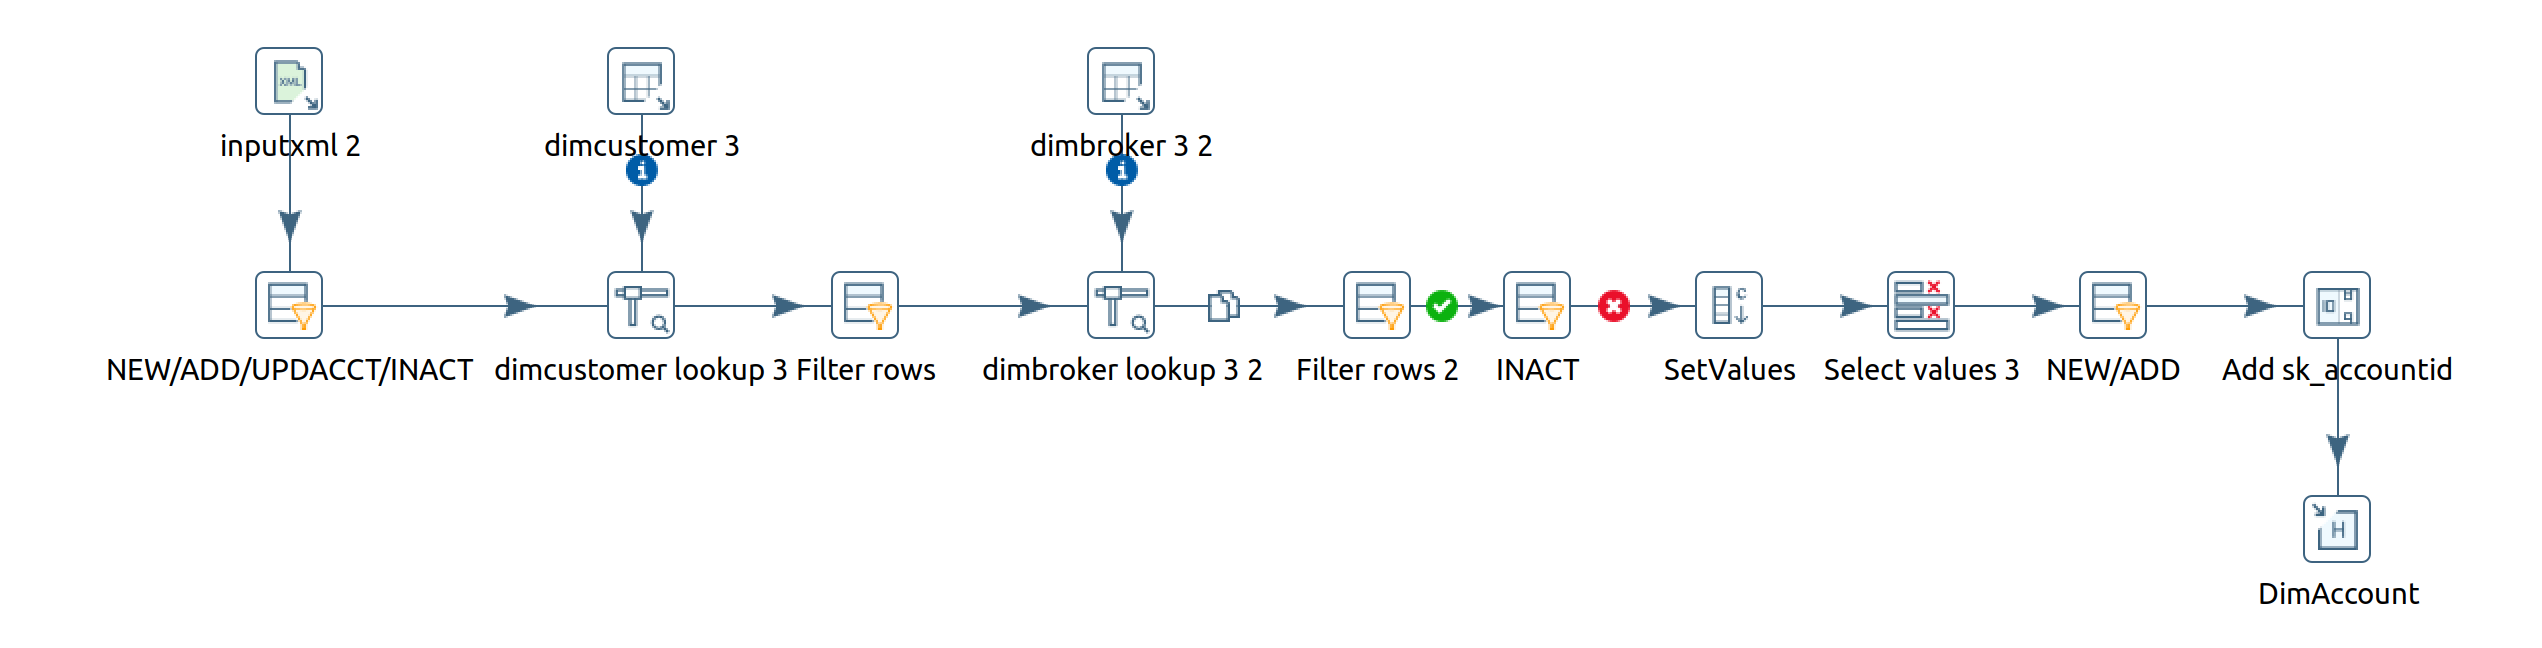
\includegraphics[width=15cm, height=6cm]{images2/DimAcc.png}
\end{center}
\caption{Implementation of DimAccount table}
\label{DimAcc}
\end{figure} 

\subsubsection{DimTrade}
DimTrade data is extracted form \pcw{TradeHistory.txt} and \pcw{Trade.txt}. On the basis of the T\_ID field, the incoming files may be logically linked. A new DimTrade record is created if a T\_ID encountered does not match a TradeID from the DimTrade table. The DimTrade record is updated when a T\_ID is found that matches one of the TradeIDs in the DimTrade database. 
\begin{figure}[H] 
\begin{center}
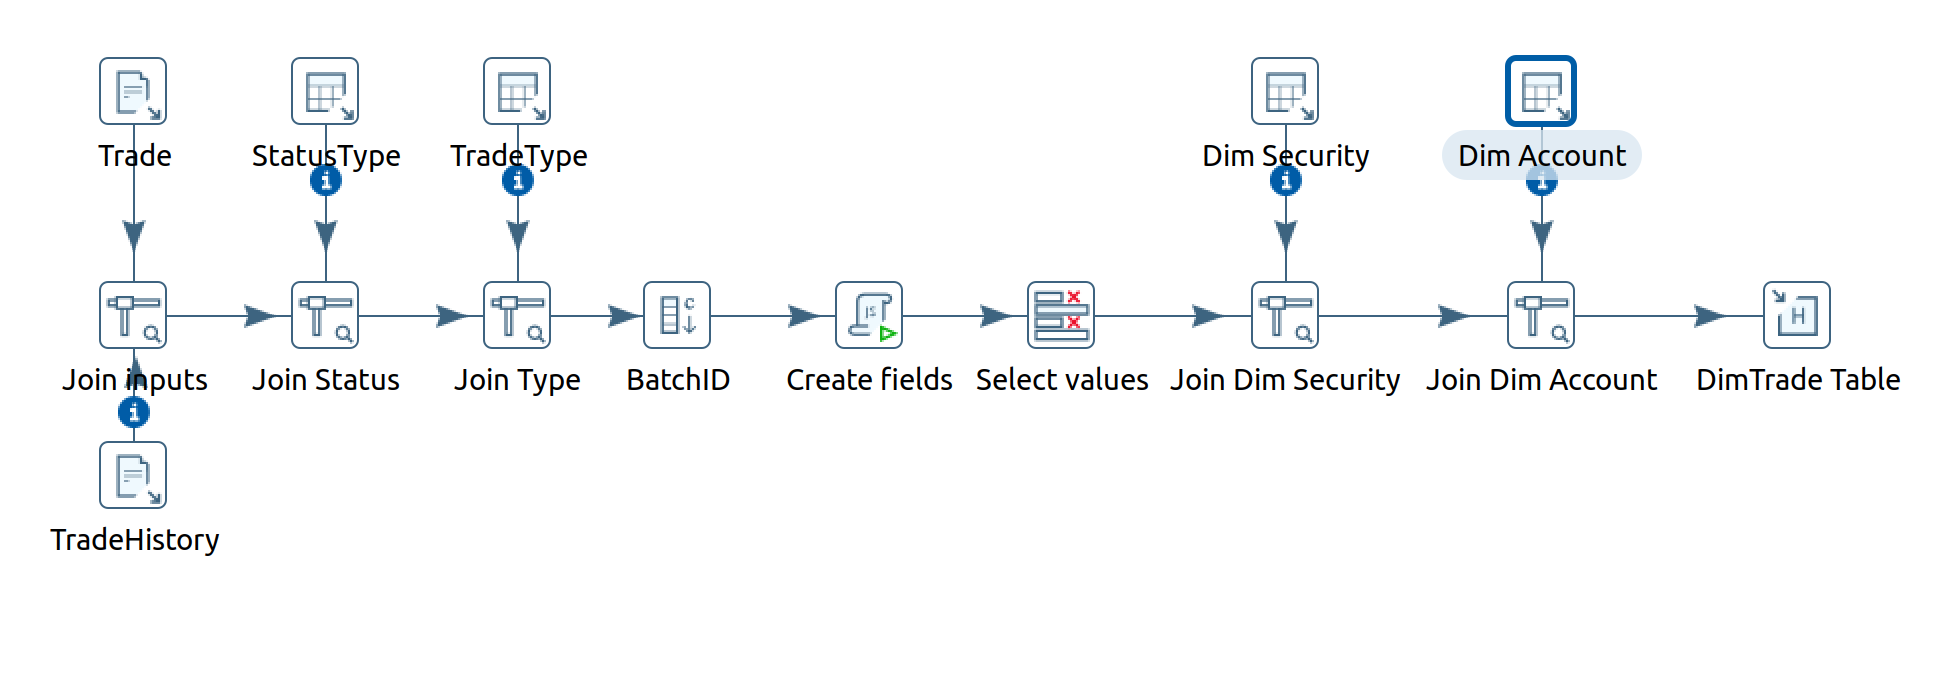
\includegraphics[width=15cm]{images2/DimTRD.png}
\end{center}
\caption{Implementation of DimTrade table}
\label{DimAcc}
\end{figure} 

\subsubsection{FactHoldings}
The \pcw{HoldingHistory.txt} file and the DimTrade table provide data for FactHoldings.
The number and price values represent a security's holdings following the most recent exchange. 
\begin{figure}[H] 
\begin{center}
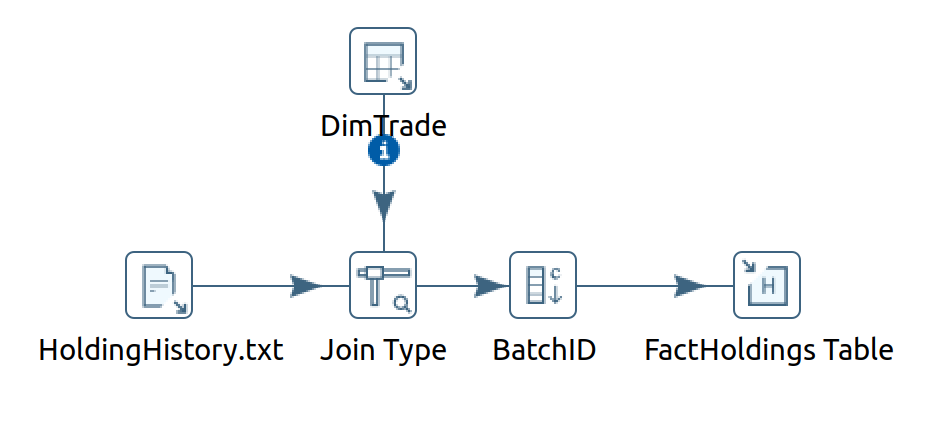
\includegraphics[width=15cm, height=6cm]{images2/factHold.png}
\end{center}
\caption{Implementation of FactHoldings table}
\label{fctHold}
\end{figure} 


\subsubsection{FactCashBalances}
FactCashBalances data is extracted from the file \pcw{CashTransaction.txt}. The net effect of all cash transactions for a specific account on a given day is summed, and only one record is created per account with changes on that day. 

\begin{figure}[H] 
\begin{center}
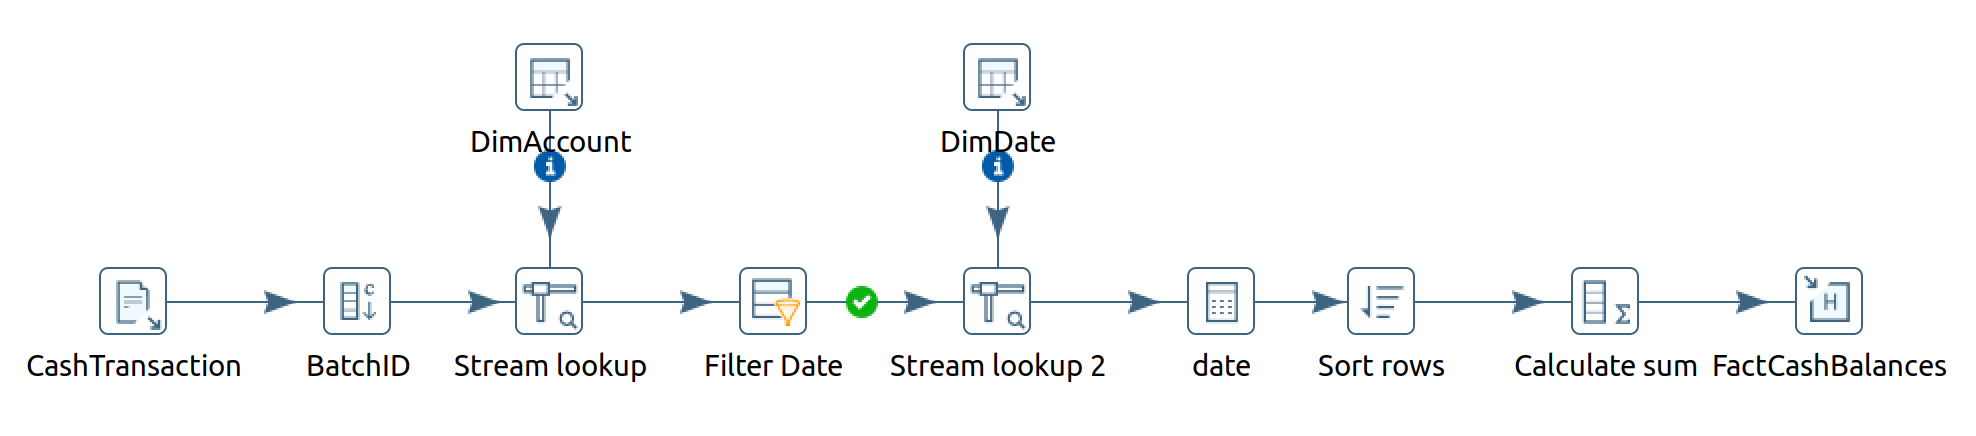
\includegraphics[width=15cm]{images2/balance.png}
\end{center}
\caption{Implementation of FactCashBalances table}
\label{fctBlc}
\end{figure} 



\subsection{Automatic Auditing}
After all ETL tasks have been completed and the database is populated. We should perform automated audit queries to verify the accuracy of all transformations. And check the accuracy and consistency of the data.

Prof. Esteban Zimanyi provided us with 4 scripts via email to audit our results. since Impala syntax and dataypes are limited and strict, it was not easy to adapted them. Thus, all 4 scripts failed.

\section{Results and benchmarks}

In this section, the different benchmarks done as well as their results and some analysis will be seen.
It has been decided to set the size of the  data-set to 1 GB. The table shows the execution time that an ETL process takes for each table and the figure illustrates the time differences.

\begin{table}[H]
\begin{center}
\begin{tabular}{|c|c|c|}
\hline
raw & Table             & Execution time \\ \hline
1   & Industry          & 0.0s           \\ \hline
2   & StatusType        & 0.0s           \\ \hline
3   & TaxRate           & 0.0s           \\ \hline
4   & TradeType         & 0.1s           \\ \hline
5   & DimDate           & 0.9s           \\ \hline
6   & DimTime           & 2.2s           \\ \hline
7   & DimBroker         & 2.5s           \\ \hline
8   & Prospect          & 3.4s            \\ \hline
9   & DimCompany        & 5.9s           \\ \hline
10  & DimSecurity       & 6.4s           \\ \hline
11  & Financial         & 14.1s          \\ \hline
12  & FactCashBalances  & 26s            \\ \hline
13  & FactWatches       & 43.2s          \\ \hline
14  & DimAccount        & 78s            \\ \hline
15  & DimTrade          & 81s            \\ \hline
16  & DimCustomer       & 88s            \\ \hline
17  & FactHoldings      & 202s           \\ \hline
18  & FactMarketHistory & 210s           \\ \hline
\end{tabular}
\end{center}
\end{table}


\begin{figure}[H]
    \centering
    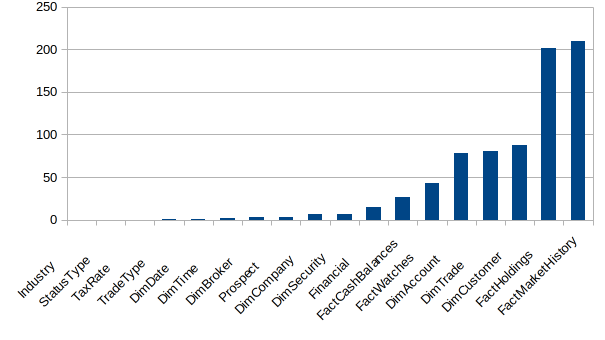
\includegraphics[width=\textwidth]{images2/img.png} 
    \caption{Execution time in seconds for each table ETL process}
\end{figure}

Note that for dimCustomer and dimAccount, only insertions have been performed. The obtained results show that it takes 10 min to perform the historical load. Thus, taking into account the updates or the modification that should be done could increase a lot the time needed.

\section{Conclusion}
In this project, \ita{TPC-DI} tools have been used in order to get a data integration benchmark of Apache Impala. In this report, the necessary steps and critical points of experimentation described so that anyone can be able to reproduce the obtained results.

A challenging thing was that the documentation for TPC-DI which had not a good quality (the last update was for 2014).

It is also noteworthy to mention that Pentaho provides an excellent services for data integration and it is really simple to work with this tool.

The main issue was the Read-Only aspect of Impala. Since we were not able to perform any Update of the Inserted Data, we could not implement some part of TPC-DI and could not perform the audit Part. However Impala is suitable for large data warehouses, as it is capable of holding terabytes of data.

\begin{thebibliography}{99}
    \bibitem{source001}
     \emph{Transaction Processing Performance Council (TPC) - TPC BENCHMARK™ DI Standard Specification — Version 1.1.0, November 2014}
    
\end{thebibliography}

\end{document}